Gerum ráð fyrir að eftirfarandi sé þekkt
\begin{itemize}
\item[$b_i$] Magn af hráefni (e. resources) með takmörkuðu framboði, til ráðstöfunar, þar sem \mbox{$i\in\{1,\ldots,m\}$}.
\item[$x_j$] Framleiðslumagn (e. activity) af afurð $j$, þar sem \mbox{$j\in\{1,\ldots,n\}$}.
\item[$c_j$] Framlegð af afurð $j$.
\item[$a_{ij}$] Magn af hráefni $i$ sem þarf til þess að framleiða afurð $j$.
\end{itemize}
Línulegt bestunarverkefni (LP) á \ath{stöðluðu} (e. standard) formi\footnote{Skv. Hillier og Lieberman} er að hámarka
\begin{equation}
\max_{x_1,\ldots,x_n}  z = \sum_{j=1}^n c_j x_j 
\end{equation}
með tilliti til skorðanna:
\begin{eqnarray}
\sum_{j=1}^n a_{ij} x_j  \le  b_i &\quad& i\in\{1,\ldots,m\} \\
x_j  \ge  0 &\quad&  j\in\{1,\ldots,n\}
\end{eqnarray}
eða á fylkjaformi:
\begin{equation}
 \max_{\mathbf{x}} z = \mathbf{c}^{T}\mathbf{x}
\end{equation}
með tilliti til skorðanna:
\begin{eqnarray}
\mathbf{A}\mathbf{x}  \le  \mathbf{b} \\
\mathbf{x} \ge  \mathbf{0}
\end{eqnarray}
\newpage
Önnur form LP verkefna eru einnig möguleg:
\begin{itemize}
 \item Lágmörkun, $\min_{\vec{x}} z$.
 \item Stærra-en skorður, $a_{i1}x_1+\cdots+1_{in}x_n\geq b_i$.
 \item Jafnt-og skorður,  $a_{i1}x_1+\cdots+1_{in}x_n = b_i$.
 \item Eitt eða fleiri $x_j$ geta verið neikvæð.
\end{itemize}
\begin{aths}
 Ólínulegum skorðum á forminu
$$ \frac{x_1}{x_2+x_3}\leq b$$
má breyta í jafngildar línulegar skorður
$$ x_1 \leq bx_2+bx_3 $$
eða
$$ x_1-bx_2-bx_3 \leq 0$$
Sjá sýnidæmi bls. 51-55 í H\&L.
\end{aths}

\begin{daemi}[Wyndor-Glass Company]\label{wyndor:org}
Wyndor glervöru\-framleiðandi ætlar að hefja framleiðslu á tveimur nýjum vörutegundum sem er hægt að framleiða þremur mismunandi verksmiðjum. 
\begin{itemize}
 \item Vara 1: Framleidd í verksmiðju 1 og 3
 \item Vara 2: Framleidd í verksmiðju 2 og 3
\end{itemize}
Hægt er að selja allt sem er framleitt. 
Eftirfarandi upplýsingar liggja fyrir:
\begin{center}{\renewcommand{\arraystretch}{1.5} \renewcommand{\tabcolsep}{0.2cm}
\begin{tabular}{|cccc|} \hline 
Verksmiðja & \multicolumn{2}{c}{Framleiðslutími (klst)} & Tími til umráðana \\
& Vara 1 & Vara 2 &  \\ \hline
1 & 1 & 0 & 4 \\
2 & 0 & 2 & 12 \\
3 & 3 & 2 & 18 \\ \hline 
Framlegð & \$3000 & \$5000 & \\ \hline
\end{tabular}

}\end{center}

Notum línulega bestun t.þ.a. ákvarða hversu mikið eigi að framleiða þannig að framlegðin sé hámörkuð.
\end{daemi}
\begin{lausn}Ákvarðanabreyturnar eru
\begin{eqnarray*}
 x_1 &=& \textrm{ magn af vöru } 1\\
x_2 &=& \textrm{ magn af vöru } 2
\end{eqnarray*}
Markfallið er 
\begin{equation}
\max_{x_1,x_2} 3x_1+5x_2 \label{wyndor:markfall} 
\end{equation}
m.t.t. skorðanna
\[\begin{array}{ccccc}
 x_1 & && \leq & 4 \\
 & &2x_2 & \leq &12 \\
 3x_1& + &2x_2&\leq&18\\
 &x_1,&x_2&\geq&0
\end{array}\]

Hér er einungis um tvær ákvarðanabreytur um að ræða, getum því fundið bestu lausn \emph{grafískt}. 
 
Viljum finna $\vec{x}^*=(x_1^*,x_2^*)$ sem hámarkar $z$. Fyrsta skrefið er að kanna hvaða gildi eru \emph{gjaldgeng} (e. feasible) þ.e. uppfylla allar skorður. Vitum að vegna þess að $x_1>0$ og $x_2>0$ þá kemur 1. fjórðungur eingungis til greina. Ytri mörk skorða (e. constraint boundary) fást m.þ.a. skipta ójöfnu út fyrir jöfnu. Til dæmis
$$ 3x_1+2x_2\leq 18 \quad \Rightarrow \quad 3x_1+2x_2=18$$
Í tveimur víddum eru þessi mörk línur.

\begin{aths}Til þess að finna hvorum megin við ytri mörkin gjaldgengar lausnir liggja, stingum við einhverjum heppilegum punkti, t.d. $(0,0)$ inn í ójöfununa og athugum hvort hún sé uppfyllt. 
\end{aths}
Því næst er að teikna hæðarlínur fyrir einhver gildi á $z$. Förum samsíða hæðalínunum í hækkandi átt (hér upp og til hægri) eins langt og kemst innan gjaldgegna svæðisins, ysti leyfilegi punkturinn er besta lausn líkansins. Sjáum á mynd \ref{wyndor:img:grafisk} að $\vec{x}^*=(2,6)$ gefur hæsta markfallsgildi, $z^*=36$.

\begin{figure}[t!]
\centering
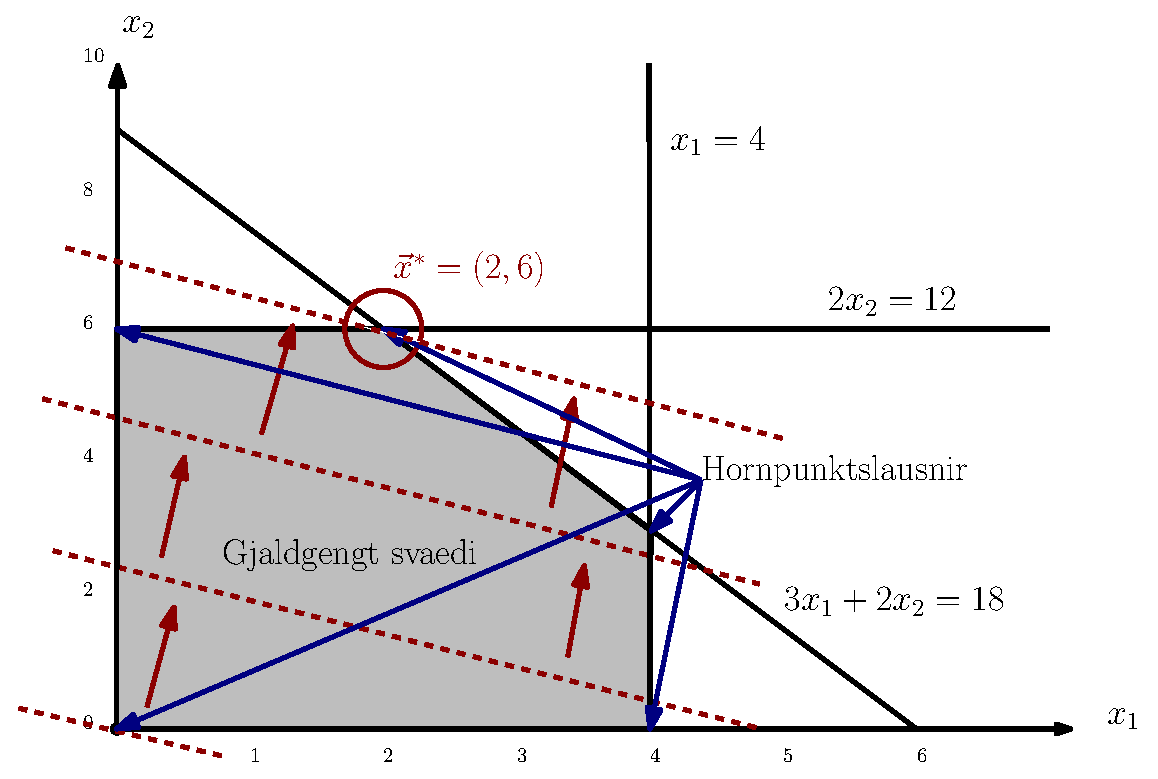
\includegraphics[width=0.7\columnwidth]{figs/wyndor_org.eps}
\caption{Myndræn lausn á dæmi \ref{wyndor:org} (Wyndor-Glass Company). Gjaldgegna svæðið afmarkast af skorðum líkansins, og hæðarlínur markfallsins $z$ eru teiknaðar sem rauðar brotalínur.}\label{wyndor:img:grafisk}
\end{figure}
\end{lausn}

\section{Nokkur hugtök}
%Til saman skilgreina skorðurnar \ath{gjaldgengt svæði} (e. feasible region) en það er mengi allra \ath{gjaldgengra lausna} (e. feasible solution).

%\ath{Besta lausn} (e. optimal solution) er sú lausn sem hámarkar (eða lágmarkar) markfallið $z$.

\begin{itemize}
\item \ath{Ákvarðanabreytur} (e. decision variables) $x_1,\ldots,x_n$
\item \ath{Ákvörðun eða lausn} (e. decision or solution) er tiltekin gildi á ákvarðana\-breytum
\item \ath{Markfall} (e. objective function) $z$
\item \ath{Gjaldgeng lausn} (e. feasible solution) er lausn sem uppfyllir skorður
\item \ath{Gjaldgengt svæði} (e. feasible region) mengi gjaldgengra lausna
\item \ath{Besta lausn} (e. optimal or best solution) er gjaldgeng lausn sem hámarkar (eða lágmarkar í $\min$  verkefni) markfall $z$
\begin{aths}
Stundum eru fleiri en ein jafngóðar bestu lausnir (jafnvel óendanlega margar, sbr. ef dæmi \ref{wyndor:org} væri með markfall samsíða skorðunni $z=3x_1+2x_2$).
\end{aths}
\item \ath{Gjaldgeng hornpunktslausn} (e. corner-point feasible solution) er lausn í hornpunkti gjaldgengs svæðis.
\end{itemize}

Lausn í hornpunkti gjaldgenga svæðisins er lausn þar sem $n$ ójöfnuskorður eru uppfylltar með $=$ merki; þær eru sagðar \athsup{virkar}{Skorður} (e. active).

Setja má fram bestunarverkefni sem hafa \ath{engar gjaldgengar lausnir} (e. infeasible).
\begin{daemi}\label{wyndor:infeasible}
Tökum dæmi \ref{wyndor:org} og bætum við skorðunni $$3x_1+5x_2\geq 50$$ þá eru skorðurnar sýndar myndrænt á mynd \ref{wyndor:img:infeasible}. Sjáum að við getum aldrei uppfyllt allar skorður samtímis, þ.a.l. engar gjaldgengar lausnir til á líkaninu.
\end{daemi}

\begin{aths}
 Þessi staða kemur stundum upp ef LP verkefni er sett ranglega fram.
\end{aths}

Annar möguleiki er að gjaldgegna svæðið sé \ath{ótakmarkað} (e. unbounded), þ.e.a.s. markfallið getur vaxið/minnkað hindrunarlaust.

\begin{daemi}\label{wyndor:unbounded}
Tökum aftur dæmi \ref{wyndor:org} og sleppum tveimur skorðum, þ.e.
$$\max_{\vec{x}}z=3x_1+5x_2$$
m.t.t. sk.
$$ x_1\leq 4$$
Sjáum á mynd \ref{wyndor:img:unbounded} að $z$ getur orðið eins stórt og vera vill.


\begin{figure}[t!]
\centering
\includegraphics[width=0.75\columnwidth]{figs/wyndor_infeasible.eps}
\caption{Myndræn lausn á dæmi \ref{wyndor:infeasible} (Wyndor-Glass Company). Gjald\-genga svæðið afmarkast af skorðum líkansins, sjáum að við getum aldrei uppfyllt allar skorður samtímis.}\label{wyndor:img:infeasible}
\includegraphics[width=0.75\columnwidth]{figs/wyndor_unbounded.eps}
\caption{Myndræn lausn á dæmi \ref{wyndor:unbounded} (Wyndor-Glass Company). Gjald\-genga svæðið afmarkast af skorðum líkansins, sjáum að $z$ getur orðið eins stórt og verða vill.}\label{wyndor:img:unbounded}
\end{figure} 
 
\end{daemi}

Athugum nú hvernig leysa má LP verkefni á skipulegan hátt. Eftirfarandi setning reynist gagnleg

\begin{setn}
Um línuleg bestunarverkefni með eina eða fleiri gjaldgengar lausnir og lausnarsvæði sem ekki eru ótakmörkuð gildir:
\begin{enumerate}
 \item Ef verkefnið hefur nákvæmlega eina bestu lausn, þá er hún í hornpunkti lausnarsvæðisins.
 \item Ef verkefnið hefur fleiri en eina bestu lausn þá eru a.m.k. tvær þeirra gjaldgengar hornpunktslausnir.
\end{enumerate}
\end{setn}
Fjöldi gjaldgengra hornpunktslausna er þar að auki endanlegur. 
Tillaga að reikniriti er því: 
Prófa allar gjaldgengar hornpunktslausnir.

\begin{aths}
 Í raunveruleikanum vex fjöldi slíkra punkta mjög hratt með fjölda ákvarðanabreyta $n$ og skorðna $m$, svo þetta reynist frekar óraunhæft reiknirit fyrir stærri verkefni.
\end{aths}


\section{Forsendur línulegrar bestunar}
Til þess að beita megi hefðbundinni línulegri bestun er gert ráð fyrir eftirfarandi forsendum:
\begin{description}
\item \ath{Hlutfallsleiki} (e. proportionality): Framlag afurðar $j$ til markfallsins er í hlutfalli við gildi á $x_j$, þ.e.a.s. $z$ er línulegt fall af ákvarðanabreytum. Sama gildir um vinstri hlið í skorðum. 
\item \ath{Samleggjanleiki} (e. additivity): Markfall og vinstri hlið skorða er summa framlaga frá einstökum afurðum.\footnote{
T.d. væri samlegðaráhrif nóg til að \emph{brjóta} þessa forsendu, sbr. \mbox{$z=3x_1+5x_2+x_1x_2$}}
\item \ath{Deilanleiki} (e. divisibility): Ákvarðanabreytur geta tekið hvaða rauntölugildi sem er innan lausnarsvæðisins.\footnote{
Ef þær þurfa að vera heiltölur þarf að nota heiltölubestun.}
\item \ath{Vissa} (e. certainty): Gerum ráð fyrir að gildi á \emph{stikum} $a_{ij}, b_i$ og $c_j$ séu að fullu þekkt (þ.e. ekki slembnir).
\end{description}

